\section{Investigating \texttt{Min-p}'s LLM-As-A-Judge Evaluations}
\label{sec:llm_as_judge_evals}

We then turned to the original paper's LLM-as-a-Judge evaluations \citep{zheng2023judging}, specifically AlpacaEval creative writing evaluations \citep{dubois2023alpacafarm}.
% LLM-as-a-judge approaches have gained prominence as a scalable alternative to human evaluations, allowing researchers to assess model outputs across more prompts and conditions than would be feasible with human annotators alone.

\subsection{Under-Specified and Indirect Methodology Hinders Reproduction and Interpretation}

\begin{figure}[t!]
    \centering
    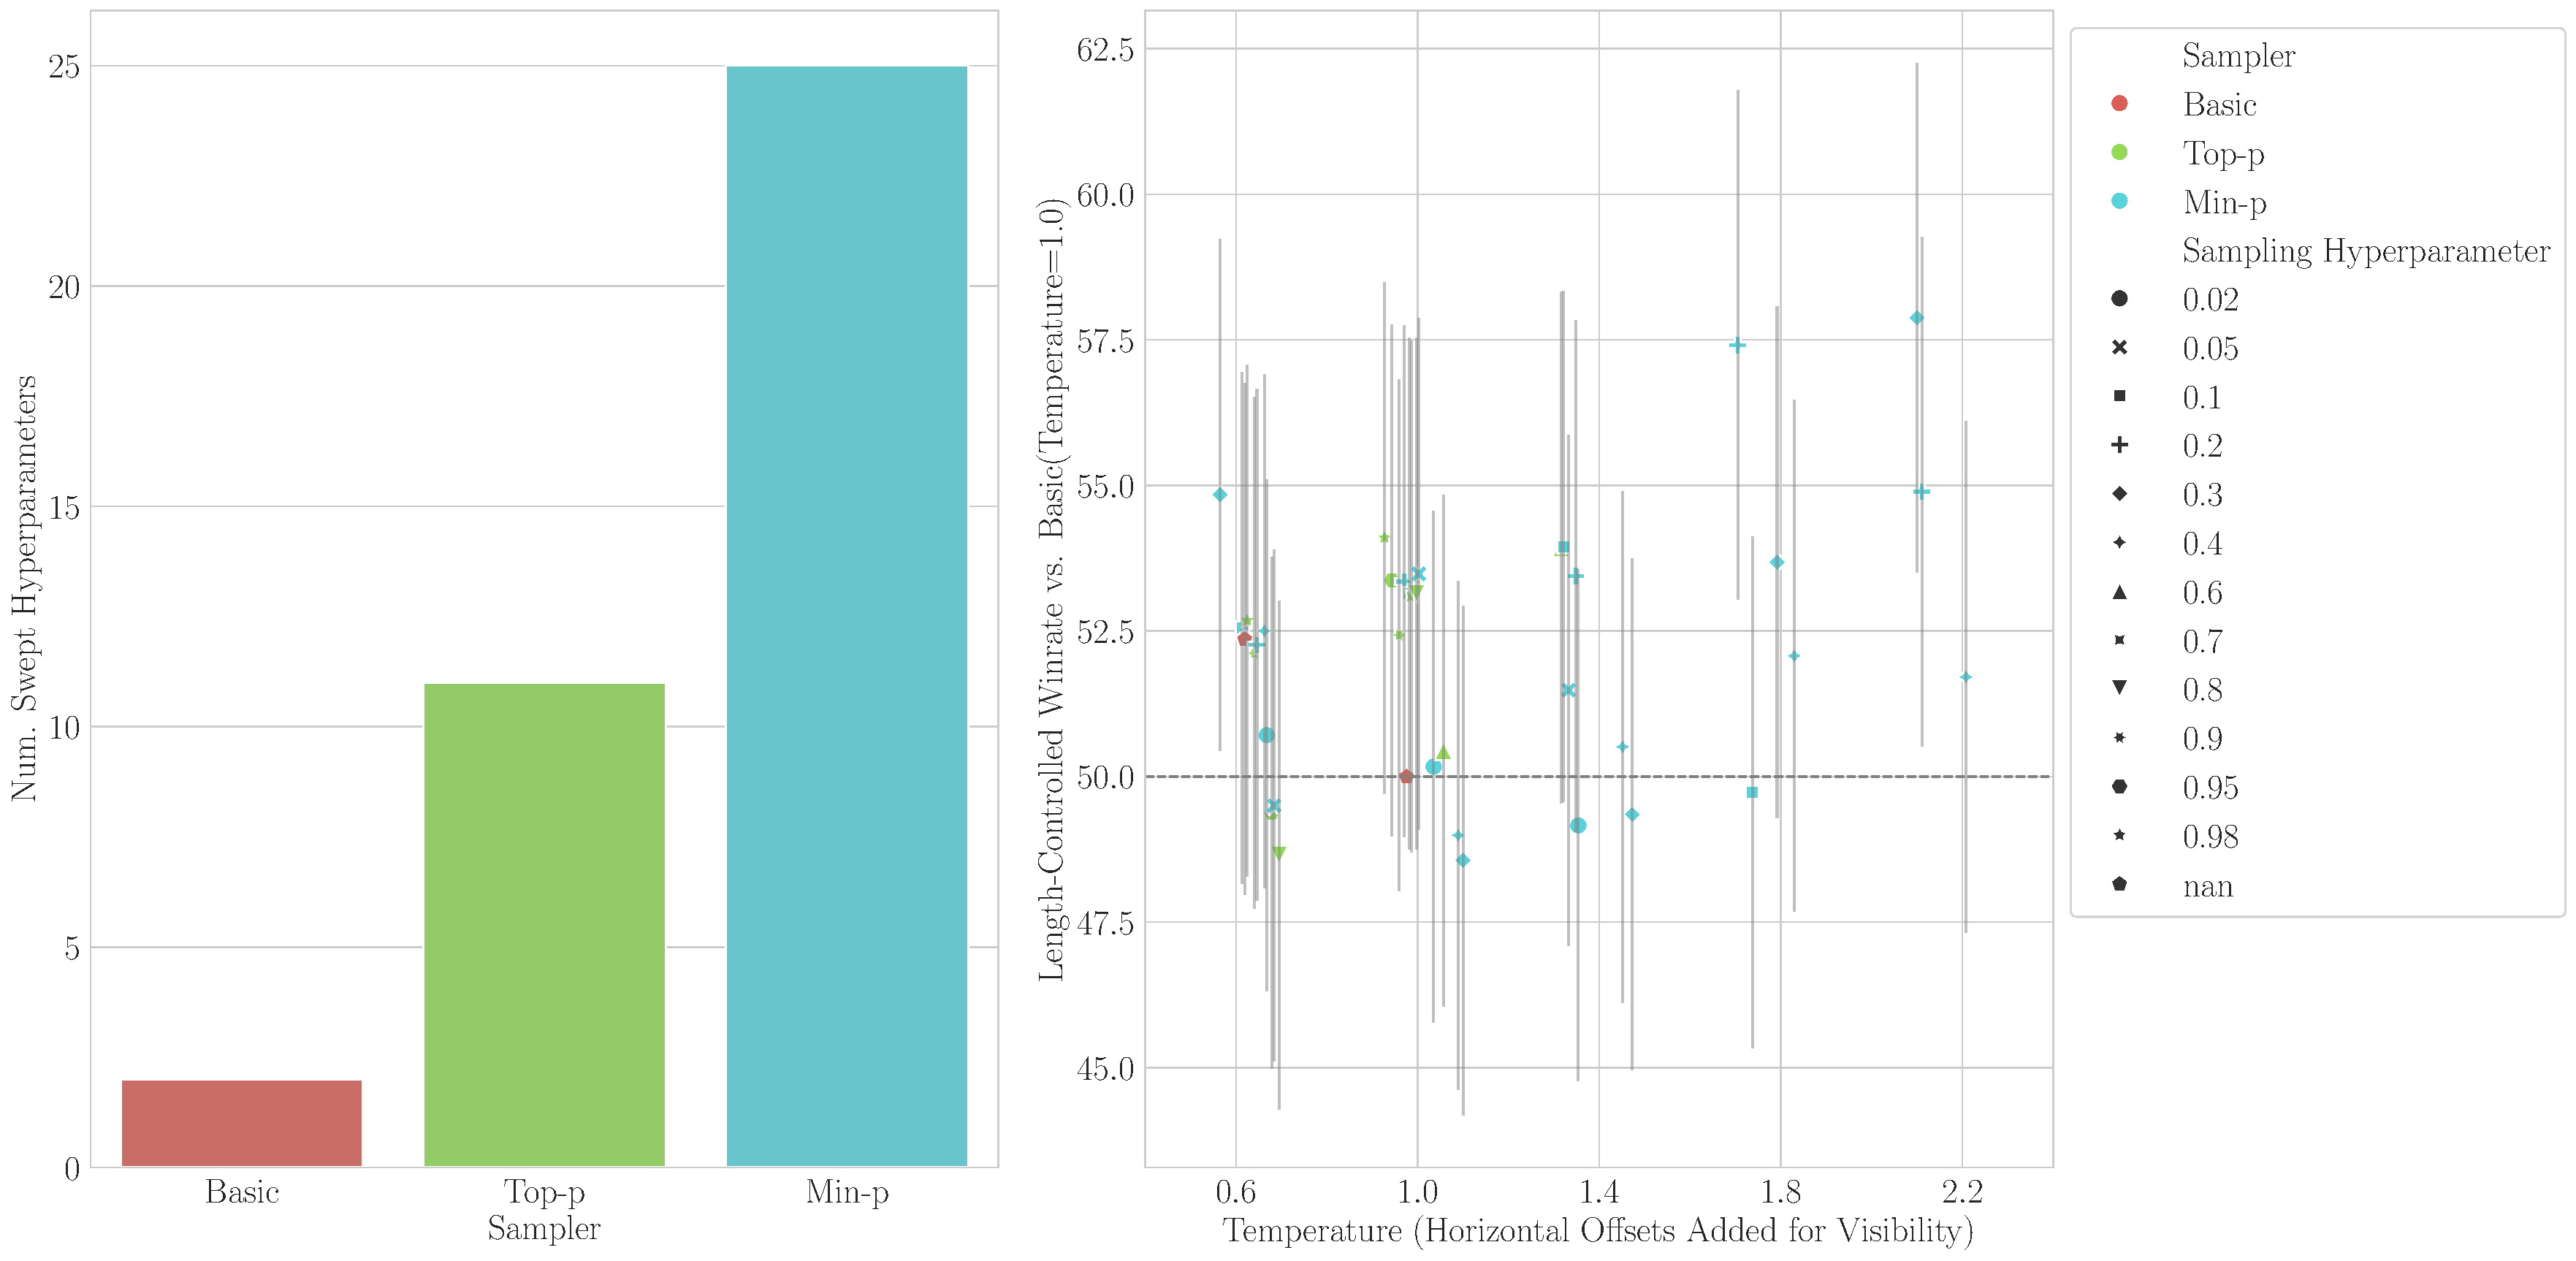
\includegraphics[width=0.9\linewidth]{figures/alpacaeval/combined_samplers_performance_plot.pdf}
    \caption{\textbf{\citet{nguyen2024minp}'s LLM-As-A-Judge Evaluations Suggest \texttt{Min-p} Typically Matches Other Samplers Despite $2\times$ to $10\times$ More Hyperparameter Tuning.} Left: \citet{nguyen2024minp} swept \texttt{min-p} with more than twice as many hyperparameters as \texttt{top-p} and more than ten times as many hyperparameters as \texttt{basic}. Right: Pairwise comparisons show \texttt{min-p} typically performs on-par with other samplers. Data were obtained from the first author's \href{https://github.com/menhguin/quest?tab=readme-ov-file}{public GitHub repository}.
    }
    \label{fig:alpacaeval}
\end{figure}


In the \href{https://arxiv.org/abs/2407.01082v2}{Oct 2024 Arxiv manuscript} and \href{https://openreview.net/notes/edits/attachment?id=SR6ORZeBAn&name=pdf}{ICLR OpenReview manuscript}, the methodology is under-specified in several ways: There is no mention which model(s) were sampled from, which model(s) served as the judge(s), or how hyperparameters were chosen or swept. Additionally, there is no description of uncertainty for the reported win rates, meaning readers are unable to decide whether win rates are statistically different from chance (50.00\%).

Furthermore, the experiment seems designed in a manner that introduces a confounder. For those unfamiliar, AlpacaEval reports win rates between paired comparisons.
Instead of directly comparing \texttt{min-p} against other samplers, the authors compared each sampler against a common fixed sampler: \texttt{basic}$(\tau=1.0)$.
This comparison strategy is indirect since comparing directly against \texttt{min-p} would offer a clearer test of its superiority while using the same number of comparisons.
The authors’ design choice is additionally concerning because LLM-judge preferences are probably not transitive, as shown by recent research \citep{xu2025investigatingnontransitivityllmasajudge}; that is, if sampler A beats sampler B, and sampler B beats sampler C, it does not necessarily follow that sampler A beats sampler C.
Therefore, comparing all methods to \texttt{basic}$(\tau=1.0)$ provides no reliable inference about \texttt{min-p}’s performance relative to \texttt{top-p} or \texttt{basic} at other temperatures. \textbf{These under-specified aspects of the methodology, combined with its indirect experimental design, make drawing conclusions difficult.}

\subsection{\texttt{Min-p} Received More Hyperparameter Tuning and Frequently Fails to Win}

No scores or code to create scores were provided with the original paper's \href{https://github.com/menhguin/minp_paper/issues/5}{GitHub repository}. While drafting this manuscript, we became aware of \href{https://github.com/IlyaGusev/quest/compare/main...menhguin:quest:main}{ongoing work} to release code in a separate repository. Results from that code revealed two discoveries: First, \texttt{min-p} received $\sim2\times$ more hyperparameter tuning than \texttt{top-p} sampling and $\sim 10\times$ more tuning than \texttt{basic} sampling (Fig.~\ref{fig:alpacaeval}, left), potentially tilting the scales in its favor. Second, the win-rates show that \texttt{min-p} frequently fails to outperform \texttt{top-p} and \texttt{basic} sampling, especially when accounting for confidence intervals; we visualized the new data with 95\% confidence intervals (with horizontal offsets added for visibility) (Fig.~\ref{fig:alpacaeval}, right).


\subsection{Table 3(b) Reported The Higher of Two Scores For \texttt{Min-p} But the Lower of Two Scores For \texttt{Top-p}}

As evidence for the LLM-As-A-Judge evaluation scores in the original paper's Table 3(b), the first author \href{https://t.me/senior_augur/76}{publicly shared a Telegram link} that showed the higher of two scores was reported for \texttt{min-p} (the reported win rate of $52.01$ corresponds to $p=0.05$, but $p=0.01$ yields a lower win rate of $50.14$) but the lower of two score was reported for \texttt{top-p} (the reported win rate of $50.07$ corresponds to $p=0.9$, but $p=0.98$ yields a higher win rate of $50.43$).
%
% \begin{itemize}
%     \item \textbf{The higher score was reported for \texttt{min-p}:} 
%     \item \textbf{The lower score was reported for \texttt{top-p}:} the reported win rate is $50.07$, corresponding to $p=0.9$. A different hyperparameter ($p=0.98$) yields a higher win rate of $50.43$.
% \end{itemize}
